\documentclass{beamer}
\mode<presentation>
\usepackage{amsmath}
\usepackage{amssymb}
%\usepackage{advdate}
\usepackage{adjustbox}
\usepackage{subcaption}
\usepackage{enumitem}
\usepackage{multicol}
\usepackage{mathtools}
\usepackage{listings}
\usepackage{float}
\usepackage{graphicx}
\usepackage{url}
\def\UrlBreaks{\do\/\do-}
\usetheme{Boadilla}
\usecolortheme{lily}
\setbeamertemplate{footline}
{
  \leavevmode%
  \hbox{%
  \begin{beamercolorbox}[wd=\paperwidth,ht=2.25ex,dp=1ex,right]{author in head/foot}%
    \insertframenumber{} / \inserttotalframenumber\hspace*{2ex} 
  \end{beamercolorbox}}%
  \vskip0pt%
}
\setbeamertemplate{navigation symbols}{}

\providecommand{\nCr}[2]{\,^{#1}C_{#2}} % nCr
\providecommand{\nPr}[2]{\,^{#1}P_{#2}} % nPr
\providecommand{\mbf}{\mathbf}
\providecommand{\pr}[1]{\ensuremath{\Pr\left(#1\right)}}
\providecommand{\qfunc}[1]{\ensuremath{Q\left(#1\right)}}
\providecommand{\sbrak}[1]{\ensuremath{{}\left[#1\right]}}
\providecommand{\lsbrak}[1]{\ensuremath{{}\left[#1\right.}}
\providecommand{\rsbrak}[1]{\ensuremath{{}\left.#1\right]}}
\providecommand{\brak}[1]{\ensuremath{\left(#1\right)}}
\providecommand{\lbrak}[1]{\ensuremath{\left(#1\right.}}
\providecommand{\rbrak}[1]{\ensuremath{\left.#1\right)}}
\providecommand{\cbrak}[1]{\ensuremath{\left\{#1\right\}}}
\providecommand{\lcbrak}[1]{\ensuremath{\left\{#1\right.}}
\providecommand{\rcbrak}[1]{\ensuremath{\left.#1\right\}}}
\theoremstyle{remark}
\newtheorem{rem}{Remark}
\newcommand{\sgn}{\mathop{\mathrm{sgn}}}
\providecommand{\abs}[1]{\left\vert#1\right\vert}
\providecommand{\res}[1]{\Res\displaylimits_{#1}} 
\providecommand{\norm}[1]{\lVert#1\rVert}
\providecommand{\mtx}[1]{\mathbf{#1}}
\providecommand{\mean}[1]{E\left[ #1 \right]}
\providecommand{\fourier}{\overset{\mathcal{F}}{ \rightleftharpoons}}
%\providecommand{\hilbert}{\overset{\mathcal{H}}{ \rightleftharpoons}}
\providecommand{\system}{\overset{\mathcal{H}}{ \longleftrightarrow}}
	%\newcommand{\solution}[2]{\textbf{Solution:}{#1}}
%\newcommand{\solution}{\noindent \textbf{Solution: }}
\providecommand{\dec}[2]{\ensuremath{\overset{#1}{\underset{#2}{\gtrless}}}}
\newcommand{\myvec}[1]{\ensuremath{\begin{pmatrix}#1\end{pmatrix}}}
\let\vec\mathbf

\lstset{
language=C,
frame=single, 
breaklines=true,
columns=fullflexible
}

\numberwithin{equation}{section}

\title{Presentation - Matgeo}
\author{Aryansingh Sonaye \\
AI25BTECH11032 \\
EE1030 - Matrix Theory}

\date{\today} 
\begin{document}

\begin{frame}
\titlepage
\end{frame}

\section{Problem}
\begin{frame}
\frametitle{Problem Statement}
\section*{Problem 3.4.1}
Draw a quadrilateral in the Cartesian plane, whose vertices are
$A(-4,5)$, $B(0,7)$, $C(5,-5)$ and $D(-4,-2)$.
\end{frame}

\section{Solution}

\subsection{Theoretical Solution }
\begin{frame}
\frametitle{Theoretical Solution}
The position vectors of the vertices are
\begin{align}
\vec{A} &= \myvec{-4\\5}, \\
\vec{B} &= \myvec{0\\7}, \\
\vec{C} &= \myvec{5\\-5}, \\
\vec{D} &= \myvec{-4\\-2}.
\end{align}
\end{frame}


\subsection{Plot}
\begin{frame}
    \frametitle{Plot}
\begin{figure}[H]
   \centering
   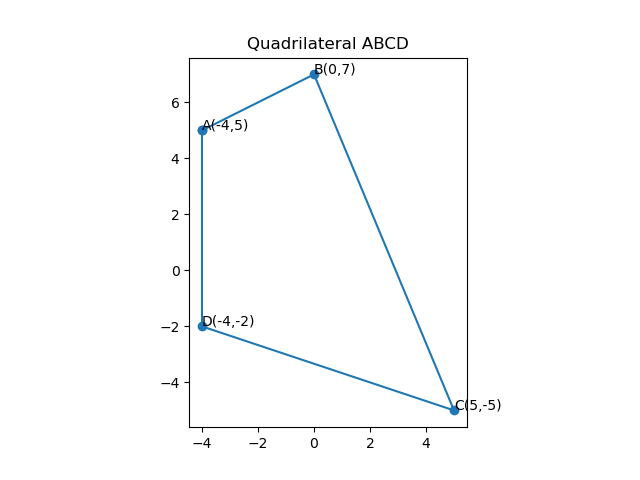
\includegraphics[width=0.9\columnwidth]{figs/quad_only.png}
   \caption{}
   \label{}
   \end{figure}
\end{frame}

\begin{frame}[fragile]
    \frametitle{Code - C}
    \begin{lstlisting}
void get_vertices(double out[8]) {
    // A(-4,5), B(0,7), C(5,-5), D(-4,-2)
    out[0] = -4.0; out[1] =  5.0;  // A
    out[2] =  0.0; out[3] =  7.0;  // B
    out[4] =  5.0; out[5] = -5.0;  // C
    out[6] = -4.0; out[7] = -2.0;  // D
}
\end{lstlisting}
\end{frame}


\begin{frame}[fragile]
    \frametitle{Code - Python(with shared C code)}
    The code to obtain the required plot is
    \begin{lstlisting}
import ctypes
import matplotlib.pyplot as plt

# 1) load the compiled C library
lib = ctypes.CDLL("./libquad.so")

# tell Python about the function signature
lib.get_vertices.argtypes = [ctypes.POINTER(ctypes.c_double * 8)]
lib.get_vertices.restype = None

# 2) create an array of 8 doubles and call C
vertices = (ctypes.c_double * 8)()
lib.get_vertices(vertices)

\end{lstlisting}
\end{frame}
\begin{frame}[fragile]
\frametitle{Code - Python(with shared C code)}
\begin{lstlisting}
# 3) convert to Python list of tuples [(x,y),...]
coords = [(vertices[i], vertices[i+1]) for i in range(0, 8, 2)]
A, B, C, D = coords

# 4) plotting
xs = [A[0], B[0], C[0], D[0], A[0]]
ys = [A[1], B[1], C[1], D[1], A[1]]

fig, ax = plt.subplots()
ax.plot(xs, ys, marker='o')


\end{lstlisting}
\end{frame}

\begin{frame}[fragile]
\frametitle{Code - Python(with shared C code)}
\begin{lstlisting}
labels = ['A(-4,5)', 'B(0,7)', 'C(5,-5)', 'D(-4,-2)']
for (x, y), lab in zip(coords, labels):
    ax.annotate(lab, (x, y))

ax.set_aspect('equal', adjustable='box')
ax.set_title('Quadrilateral ABCD')
plt.savefig("quad_only.png")
plt.show()
\end{lstlisting}
\end{frame}

\begin{frame}[fragile]
\frametitle{Code - Python only}
\begin{lstlisting}
import matplotlib.pyplot as plt

# vertices
A = (-4, 5)
B = (0, 7)
C = (5, -5)
D = (-4, -2)

# polygon coordinates (close by repeating A at end)
xs = [A[0], B[0], C[0], D[0], A[0]]
ys = [A[1], B[1], C[1], D[1], A[1]]
\end{lstlisting}
\end{frame}
\begin{frame}[fragile]
\frametitle{Code - Python only}
\begin{lstlisting}
# plot
fig, ax = plt.subplots()
ax.plot(xs, ys, marker='o')
labels = ['A(-4,5)', 'B(0,7)', 'C(5,-5)', 'D(-4,-2)']
for (x, y), lab in zip([A, B, C, D], labels):
    ax.annotate(lab, (x, y))

ax.set_aspect('equal', adjustable='box')
ax.set_title('Quadrilateral ABCD')

# save and show
out_file = "quad.png"
plt.savefig(out_file)
plt.show()

print("Saved image to", out_file)


\end{lstlisting}
\end{frame}

\end{document}
